\documentclass[12pt]{standalone}
\usepackage{tikz}
\usetikzlibrary{automata,positioning}
\begin{document}
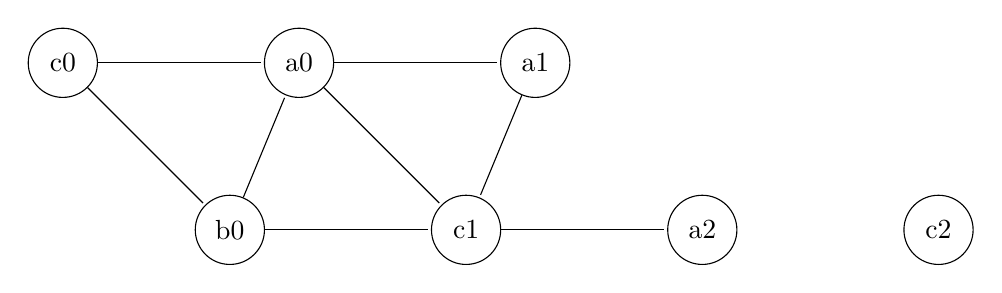
\begin{tikzpicture}[shorten >=1pt,node distance=3cm,on grid,auto] 
   \node[state] (c0)   {c0}; 
   \node[state] (b0) [below right=of c0] {b0}; 
   \node[state] (a0) [right=of c0] {a0}; 
   \node[state] (a1) [right=of a0] {a1}; 
   \node[state](c1) [below right=of a0] {c1};
   \node[state](a2) [ right=of c1] {a2};
   \node[state](c2) [right=of a2] {c2};
   
    \path[-] (c0) edge  node {} (a0);
    \path[-] (c0) edge  node {} (b0);


    \path[-] (a0) edge  node {} (c1);
    \path[-] (a0) edge  node {} (a1);
    
    \path[-] (b0) edge  node {} (a0);
    \path[-] (b0) edge  node {} (c1);

    
    \path[-] (a1) edge  node {} (c1);
    
    \path[-] (c1) edge  node {} (a2);
\end{tikzpicture}
\end{document}  
